
  % \begin{tikzpicture}[scale=0.7]
  %     \draw
  %       (-6.545, 0.0) node[draw=cyan, rounded corners] (0){Source}
  %       (-2.545, 1.2) node[draw=red, dashed, rounded corners] (1){$u$}
  %       (-2.545, 0.0) node[draw=red, dashed, rounded corners] (2){$u$}
  %       (-2.545, -1.2) node[draw=red, dashed, rounded corners] (3){$u$}
  %       (1.455, 3.0) node[draw=blue, dotted, rounded corners] (4){$v$}
  %       (1.455, 1.8) node[draw=blue, dotted, rounded corners] (5){$v$}
  %       (1.455, 0.6) node[draw=blue, dotted, rounded corners] (6){$v$}
  %       (1.455, -0.6) node[draw=blue, dotted, rounded corners] (7){$v$}
  %       (1.455, -1.8) node[draw=blue, dotted, rounded corners] (8){$v$}
  %       (1.455, -3.0) node[draw=blue, dotted, rounded corners] (9){$v$}
  %       (5.455, 0.0) node[draw=cyan, rounded corners] (10){Target};
  %     \begin{scope}[-]
  %       \draw[lightgray, text=black, font=\footnotesize]  (0) to node[]{0} (1);
  %       \draw[lightgray, text=black, font=\footnotesize]  (0) to  node[]{0} (2);
  %       \draw[lightgray, text=black, font=\footnotesize]  (0) to node[]{0}  (3);
  %       \draw[lightgray, text=black, font=\footnotesize]  (1) to  node[]{1} (4);
  %       \draw[lightgray, text=black, font=\footnotesize]  (2) to  node[]{2} (6);
  %       \draw[lightgray, text=black, font=\footnotesize]  (3) to  node[]{4} (9);
  %       \draw[lightgray, text=black, font=\footnotesize]  (4) to  node[]{0} (10);
  %       \draw[lightgray, text=black, font=\footnotesize]  (6) to  node[]{0} (10);
  %       \draw[lightgray, text=black, font=\footnotesize]  (9) to  node[]{0} (10);
  %     \end{scope}
  %   \end{tikzpicture}
    
\resizebox{0.5\textwidth}{!}{%
 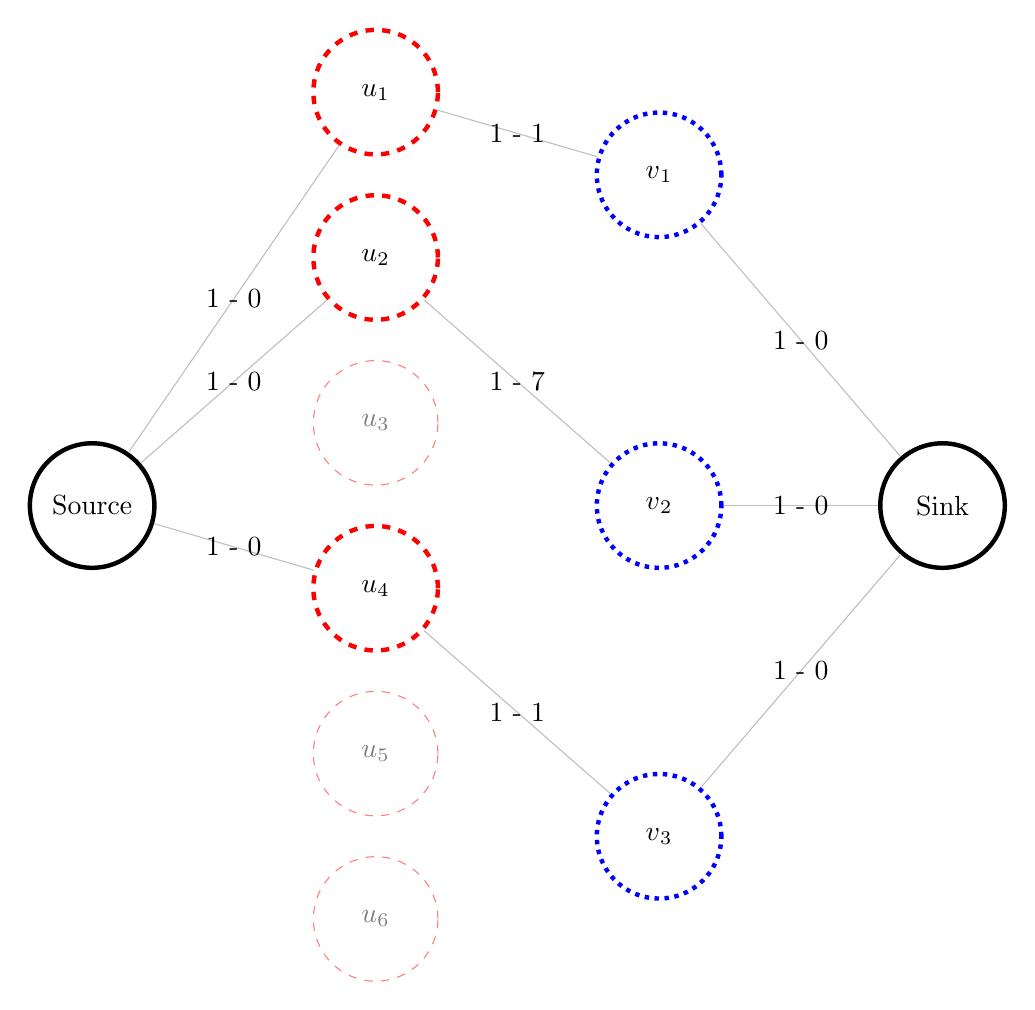
\begin{tikzpicture}[xscale=0.45,yscale=1.05]
    \tikzstyle{style} = [circle, ultra thick, draw, draw, minimum size=45pt, inner sep=0pt, text centered]
    \tikzstyle{no_border} = [circle, draw, minimum size=45pt, inner sep=0pt, text centered, opacity=0.5]


      \draw
        (-10.909, 0.0) node[style, draw=black] (0){Source}
        (-2.909, 5.0) node[style, draw=red, dashed] (1){$u$$_1$}
        (-2.909, 3.0) node[style, draw=red, dashed] (2){$u$$_2$}
        (-2.909, 1.0) node[no_border, draw=red, dashed] (3){$u$$_3$}
        (-2.909, -1) node[style, draw=red, dashed] (4){$u$$_4$}
        (-2.909, -3.0) node[no_border, draw=red, dashed] (5){$u$$_5$}
        (-2.909, -5.0) node[no_border, draw=red, dashed] (6){$u$$_6$}
        (5.091, 4) node[style, draw=blue, dotted] (7){$v$$_1$}
        (5.091, -4.0) node[style, draw=blue, dotted] (8){$v$$_3$}
        (5.091, 0) node[style, draw=blue, dotted] (9){$v$$_2$}
        (13.091, 0.0) node[style, draw=black] (10){Sink};
    
      \begin{scope}[-]
        \draw[lightgray, text=black, font=\normalsize] (0) to node[] {1 - 0} (1);
        \draw[lightgray, text=black, font=\normalsize] (0) to node[] {1 - 0} (2);
        \draw[transparent] (0) to node[] {0 - 0} (3);
        \draw[lightgray, text=black, font=\normalsize] (0) to node[] {1 - 0} (4);
        \draw[transparent] (0) to node[] {0 - 0} (5);
        \draw[transparent] (0) to node[] {0 - 0} (6);
        \draw[lightgray, text=black, font=\normalsize] (1) to node[] {1 - 1} (7);
        \draw[lightgray, text=black, font=\normalsize] (2) to node[] {1 - 7} (9);
        \draw[transparent] (3) to node[] {0 - 7} (9);
        \draw[lightgray, text=black, font=\normalsize] (4) to node[] {1 - 1} (8);
        \draw[transparent] (5) to node[] {0 - 10} (9);
        \draw[transparent] (5) to node[] {0 - 10} (8);
        \draw[transparent] (6) to node[] {0 - 10} (7);
        \draw[lightgray, text=black, font=\normalsize] (7) to node[] {1 - 0} (10);
        \draw[lightgray, text=black, font=\normalsize] (8) to node[] {1 - 0} (10);
        \draw[lightgray, text=black, font=\normalsize] (9) to node[] {1 - 0} (10);
      \end{scope}
    \end{tikzpicture}
}%